\documentclass[border=3pt]{standalone}
\usepackage{tikz}
\usetikzlibrary{arrows.meta,calc}
\tikzset{pin/.style={-{Stealth[length=5pt]}},
  blk/.style={draw, thick, minimum width=20mm, minimum height=26mm, font=\sffamily\small}}
\begin{document}
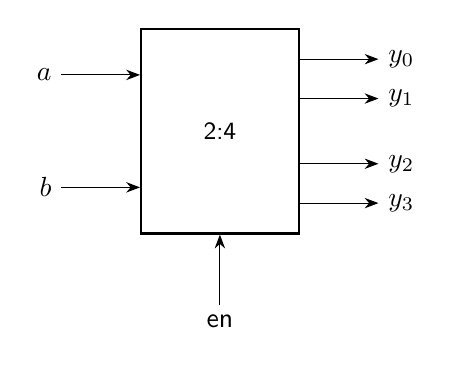
\begin{tikzpicture}[font=\sffamily]
  \node[blk] (d) {2:4};
  \draw[pin] ($(d.north west)+(-10mm,-6mm)$) node[left]{$a$} -- ($(d.north west)+(0,-6mm)$);
  \draw[pin] ($(d.south west)+(-10mm,6mm)$) node[left]{$b$} -- ($(d.south west)+(0,6mm)$);
  \draw[pin] ($(d.north east)+(0,-4mm)$) -- ++(10mm,0) node[right]{$y_0$};
  \draw[pin] ($(d.north east)+(0,-9mm)$) -- ++(10mm,0) node[right]{$y_1$};
  \draw[pin] ($(d.south east)+(0,9mm)$) -- ++(10mm,0) node[right]{$y_2$};
  \draw[pin] ($(d.south east)+(0,4mm)$) -- ++(10mm,0) node[right]{$y_3$};
  \draw[pin] ($(d.south)+(0,-9mm)$) node[below]{en} -- (d.south);
\end{tikzpicture}
\end{document}
